\documentclass[utf8]{beamer}

\usepackage[utf8]{inputenc}
\usepackage[T1]{fontenc}
\usepackage[english]{babel}

% TODO: review fonts!
\usefonttheme[onlymath]{serif}

\usetheme{default}
\title[When PageRank fails]{Ranking nodes in growing networks: \\ When PageRank fails}
\author[De Nicolao]{Pietro De Nicolao \\ \texttt{pietro.denicolao@mail.polimi.it}}
\date{\today} % TODO change
\institute{Politecnico di Milano}

% \AtBeginSection[]
% {
%   \begin{frame}<beamer>{Outline}
%     \tableofcontents[currentsection]
%   \end{frame}
% }

\begin{document}

\begin{frame}
 \titlepage
\end{frame}

\section*{Outline}
\begin{frame}
 \tableofcontents
\end{frame}

\section{Introduction}
\begin{frame}{Paper}
    \begin{center}
    \emph{\Large Ranking nodes in growing networks: \\ When PageRank fails}
    \end{center}

    Manuel Sebastian Mariani, Matúš Medo \& Yi-Cheng Zhang

    Published on \emph{Nature Scientific Reports} on 10 November 2015.
\end{frame}

\begin{frame}{PageRank}
    \begin{itemize}
        \item PageRank: most popular ranking algorithm for unipartite directed networks.
        \item Invented for Google's search algorithm, used for many other applications:
        \begin{itemize}
            \item ranking of scholarly papers
            \item ranking of images in search
            \item ranking of urban roards according to traffic flow
            \item ranking in protein interaction network
            \item etc.
        \end{itemize}
        \item \emph{A node is important if it is pointed by other important nodes.}
    \end{itemize}
    \[
        p_{ij} = (1-\gamma) \frac{w_{ij}}{s_i^{out}} + \gamma \frac{1}{N}
    \]
\end{frame}

\begin{frame}{One PageRank fits all?}
    What is the relation between PageRank's efficacy and the properties of the network?
    \begin{itemize}
        \item PageRank: \alert{static} approach
        \begin{itemize}
            \item PageRank discards temporal information
            \item works as if nodes appear all at the same time
            \item well-known bias towards old nodes
        \end{itemize}
        \item Theoretical models and real networks can exhibit \\ \alert{strong temporal patterns}.
    \end{itemize}
    \begin{center}
        \emph{Are there circumstances under which \\ the algorithm is doomed to fail?}
    \end{center}
\end{frame}

\section{Relevance Model}
\begin{frame}{The Relevance Model (RM)}
    \begin{itemize}
        \item What is the Relevance Model?
        \begin{itemize}
            \item Growing directed network model \\ with \alert{preferential attachment} and \alert{relevance}.
            \item Generalizes the classical \emph{Barabasi-Albert} model
        \end{itemize}

        \item Why using RM?
        \begin{itemize}
            \item model that best explains the linking patterns in real information systems
            \item used to model WWW, citation and technological networks
        \end{itemize}

        \item Fundamental features:
        \begin{enumerate}
            \item preferential attachment
            \item node fitness
            \item relevance and activity
            \item temporal decay
        \end{enumerate}
    \end{itemize}
\end{frame}

\begin{frame}{Relevance Model features}
    \begin{enumerate}
        \item \alert{Preferential attachment}
        \begin{itemize}
            \item similar to the Barabasi-Albert model
            \item Matthew effect: the rich get richer
            \item significant difference: \emph{existing nodes also create new links}
        \end{itemize}

        \item \alert{Fitness}
        \begin{itemize}
            \item quality parameter assigned to each node
            \item \emph{node’s inherent competence in attracting new incoming links}
        \end{itemize}

        \item \alert{Relevance and activity}
        \begin{itemize}
            \item Relevance: capacity of attracting new links over time
            \item Activity: rate at which the node generates new outgoing links
        \end{itemize}

        \item \alert{Temporal decay}
        \begin{itemize}
            \item Relevance and activity both decay with time
            \item Monotonous functions
            \item Nodes lose relevance over time
        \end{itemize}
    \end{enumerate}
\end{frame}

\begin{frame}{Generation algorithm}
    At each time $t$, the generation algorithm proceeds as follows:
    \begin{enumerate}
        \item a new node is created and connected to an existing node $i$, chosen with probability $\Pi_i^{in}(t)$.
        \item $m=10$ existing nodes are sequentially chosen \\ with probability $\Pi_i^{out}(t)$
        \begin{itemize}
            \item each selected node creates one outgoing link
            \item it selects a node $j$ as a target with probability $\Pi_j^{in}(t)$
        \end{itemize}
    \end{enumerate}
\end{frame}

\begin{frame}{Link generation}
    When a node $j$ generates a new link at time $t$, the probability that the target is node $i$ is:
    \[
        \Pi_i^{in}(t) \sim (k_i^{in}(t) + 1)\eta_i f_R (t-\tau_i)
    \]
    \begin{itemize}
        \item $k_i^{in}(t)$: current indegree of node $i$
        \item $\eta_i$: fitness of $i$
        \item $\tau_i$: time at which $i$ enters the network
        \item $f_R$: monotonously decaying function of time
        \item $R_i(t) := \eta_i f_R (t-\tau_i)$: \alert{relevance} of node $i$ at time $t$.
    \end{itemize}
\end{frame}

\begin{frame}{Node activity}
    Nodes continue being active and generate outgoing links continually.

    Probability of being chosen as an \emph{active} node at time $t$:
    \[
        \Pi_i^{out}(t) \sim A_i f_A (t-\tau_i)
    \]
    \begin{itemize}
        \item $A_i$: activity parameter
        \item $\tau_i$: time at which $i$ enters the network
        \item $f_A$: monotonously decaying function of time
        \item broad $A_i$ distribution $\Longrightarrow$ broad outdegree distribution
    \end{itemize}
\end{frame}

\begin{frame}{Effects of relevance decay}
\begin{itemize}
    \item \alert{Slow} or absent relevance decay
    \begin{itemize}
        \item recent nodes receive few links because of preferential attachment
        \item PageRank's bias towards old nodes
    \end{itemize}
    \item \alert{Fast} relevance decay
    \begin{itemize}
        \item preferential attachment compensated by decay of relevance of old nodes
        \item recent nodes can reach high indegree
        \item recent nodes mostly point to other recent nodes, because of relevance decay of older nodes
        \item old nodes point to nodes of every age because of activity
    \end{itemize}
\end{itemize}
% Figure 1 ?
\end{frame}

\begin{frame}{What makes a ranking algorithm ``good''?}
    \begin{center}
        \emph{A good ranking algorithm is expected to produce \\ an unbiased ranking where both \alert{recent} and \alert{old} nodes \\ have \alert{the same chance to appear at the top}.}
    \end{center}
    \begin{itemize}
        \item In growing networks with temporal effects, \alert{PageRank can fail} to achieve this.
    \end{itemize}
\end{frame}

\begin{frame}{PageRank time bias: numerical simulation of RM}
    \begin{figure}
        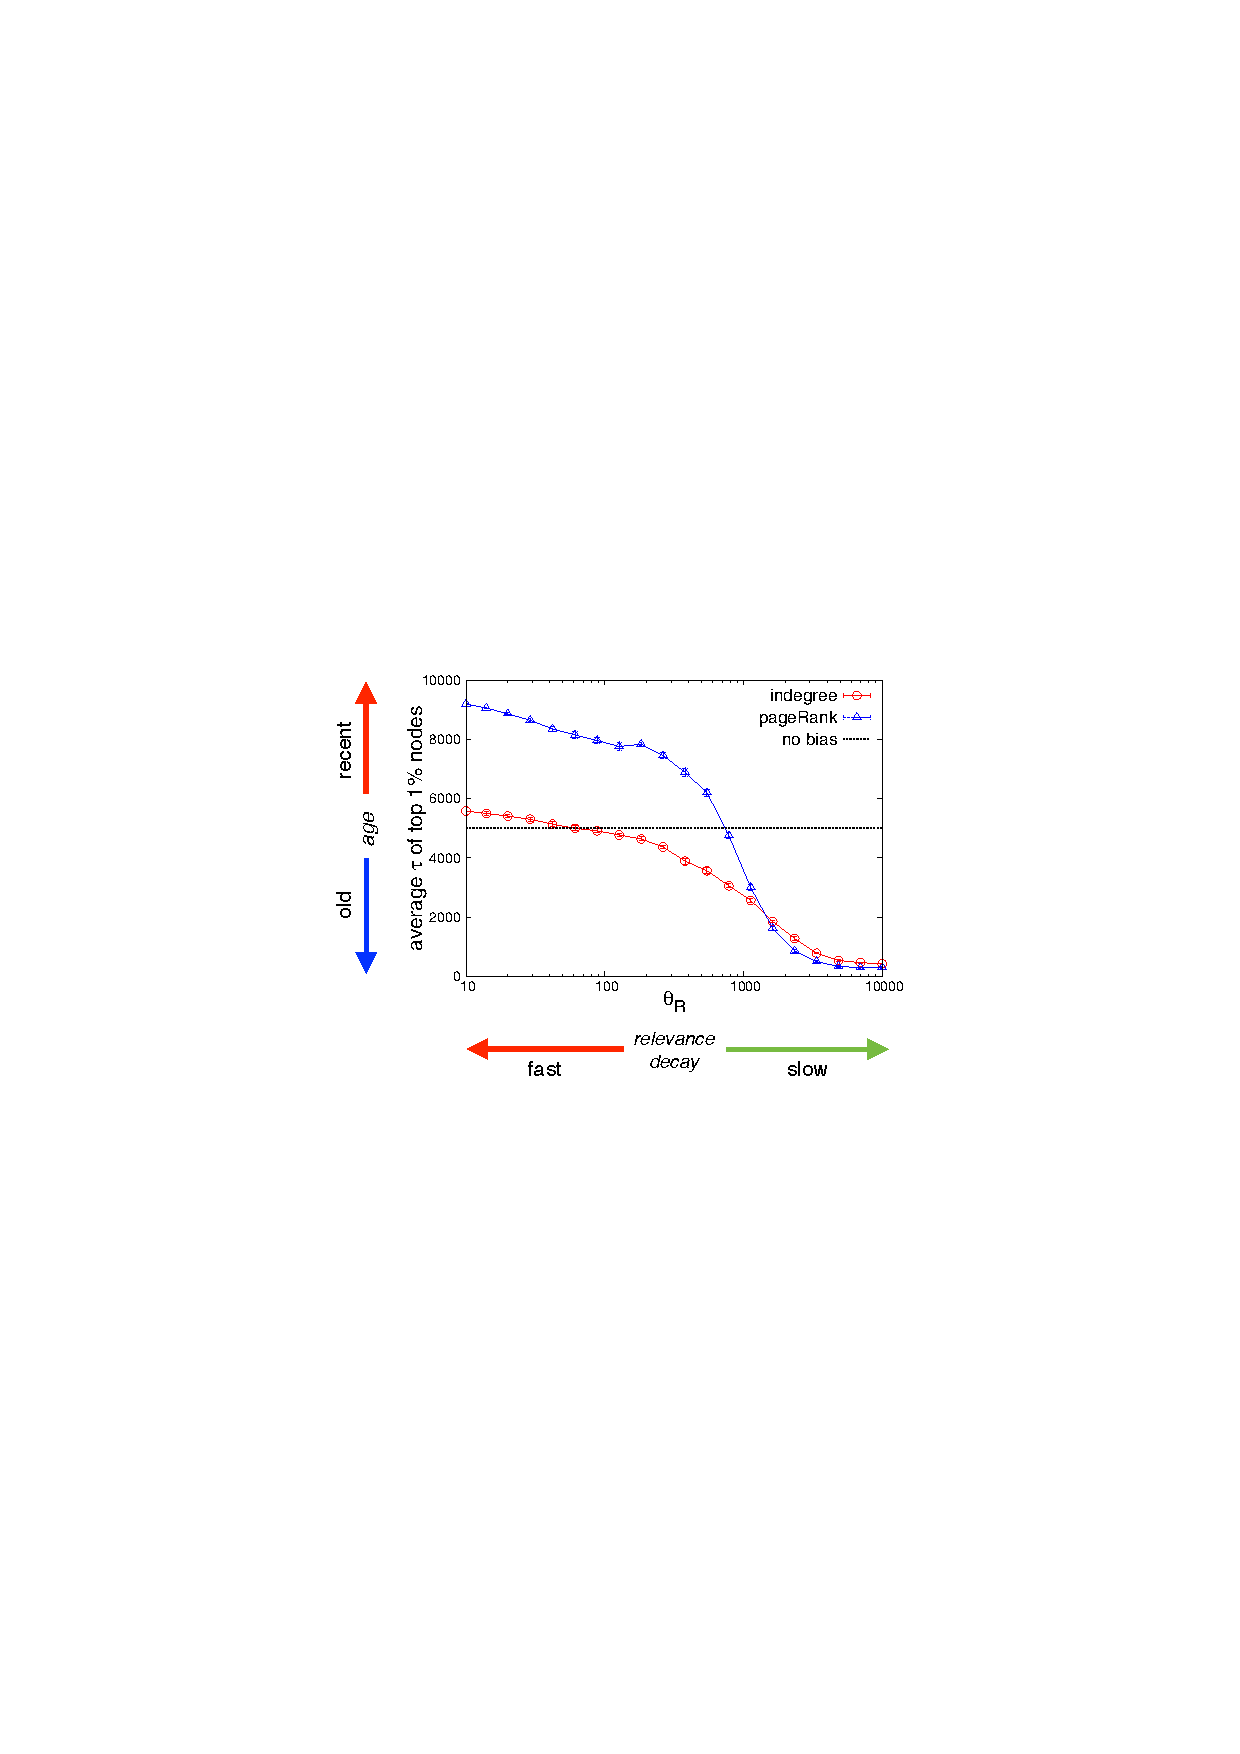
\includegraphics[width=0.7\textwidth]{figures/PageRank_time_bias}
        \caption{Comparison of PageRank and indegree rankings in the RM model. \newline
        Relevance decays as $f_R(t) = \exp(-\frac{t}{\theta_R})$. \newline
        Activity also decays exponentially, but very slowly ($\theta_A=N$).}
    \end{figure}
\end{frame}

\begin{frame}{PageRank vs. indegree: correlation with fitness}
    \begin{figure}
        \begin{columns}

        \column{0.6\textwidth}
            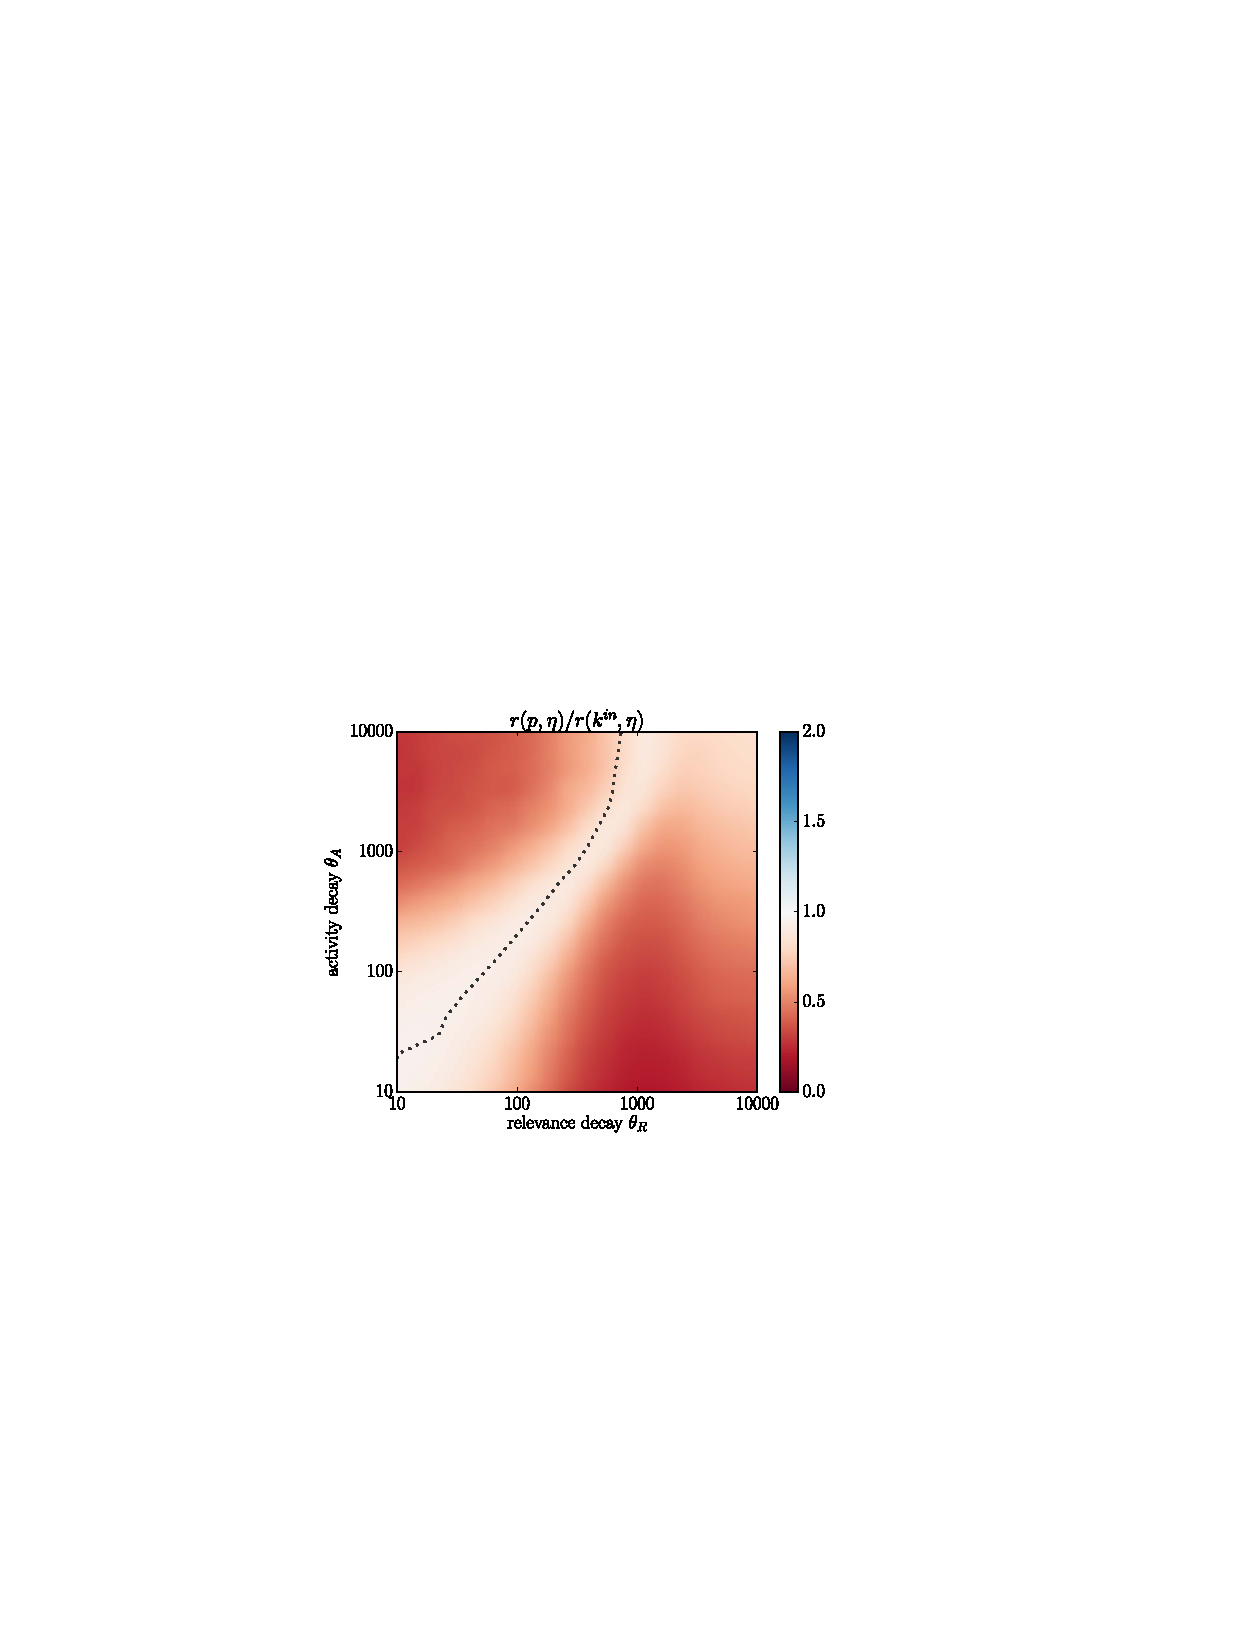
\includegraphics[width=1.0\textwidth]{figures/PageRankRM_heatmap}

        \column{0.4\textwidth}
            \caption{Comparison of performance of PageRank and indegree (RM data). \newline
            PageRank yields no improvement with respect to indegree.}
        \end{columns}
    \end{figure}
    \begin{itemize}
        \item $r(p, \eta)$: Pearson's correlation PageRank-fitness
        \item $r(k^{in}, \eta)$: Pearson's correlation indegree-fitness
        \item $\rho(\eta) = \exp(-\eta)$
    \end{itemize}
\end{frame}
\end{document}
